
\section{Usage Scenario}

In this section, we use two usage scenarios to demonstrate how AVIST support an analyst for visual exploration of big data, to identify hidden patterns, infer and verify new hypothesis.


\subsection{Network Flow Analysis} %Cyber Security Analysis

\begin{figure*}[htb]
	\centering
	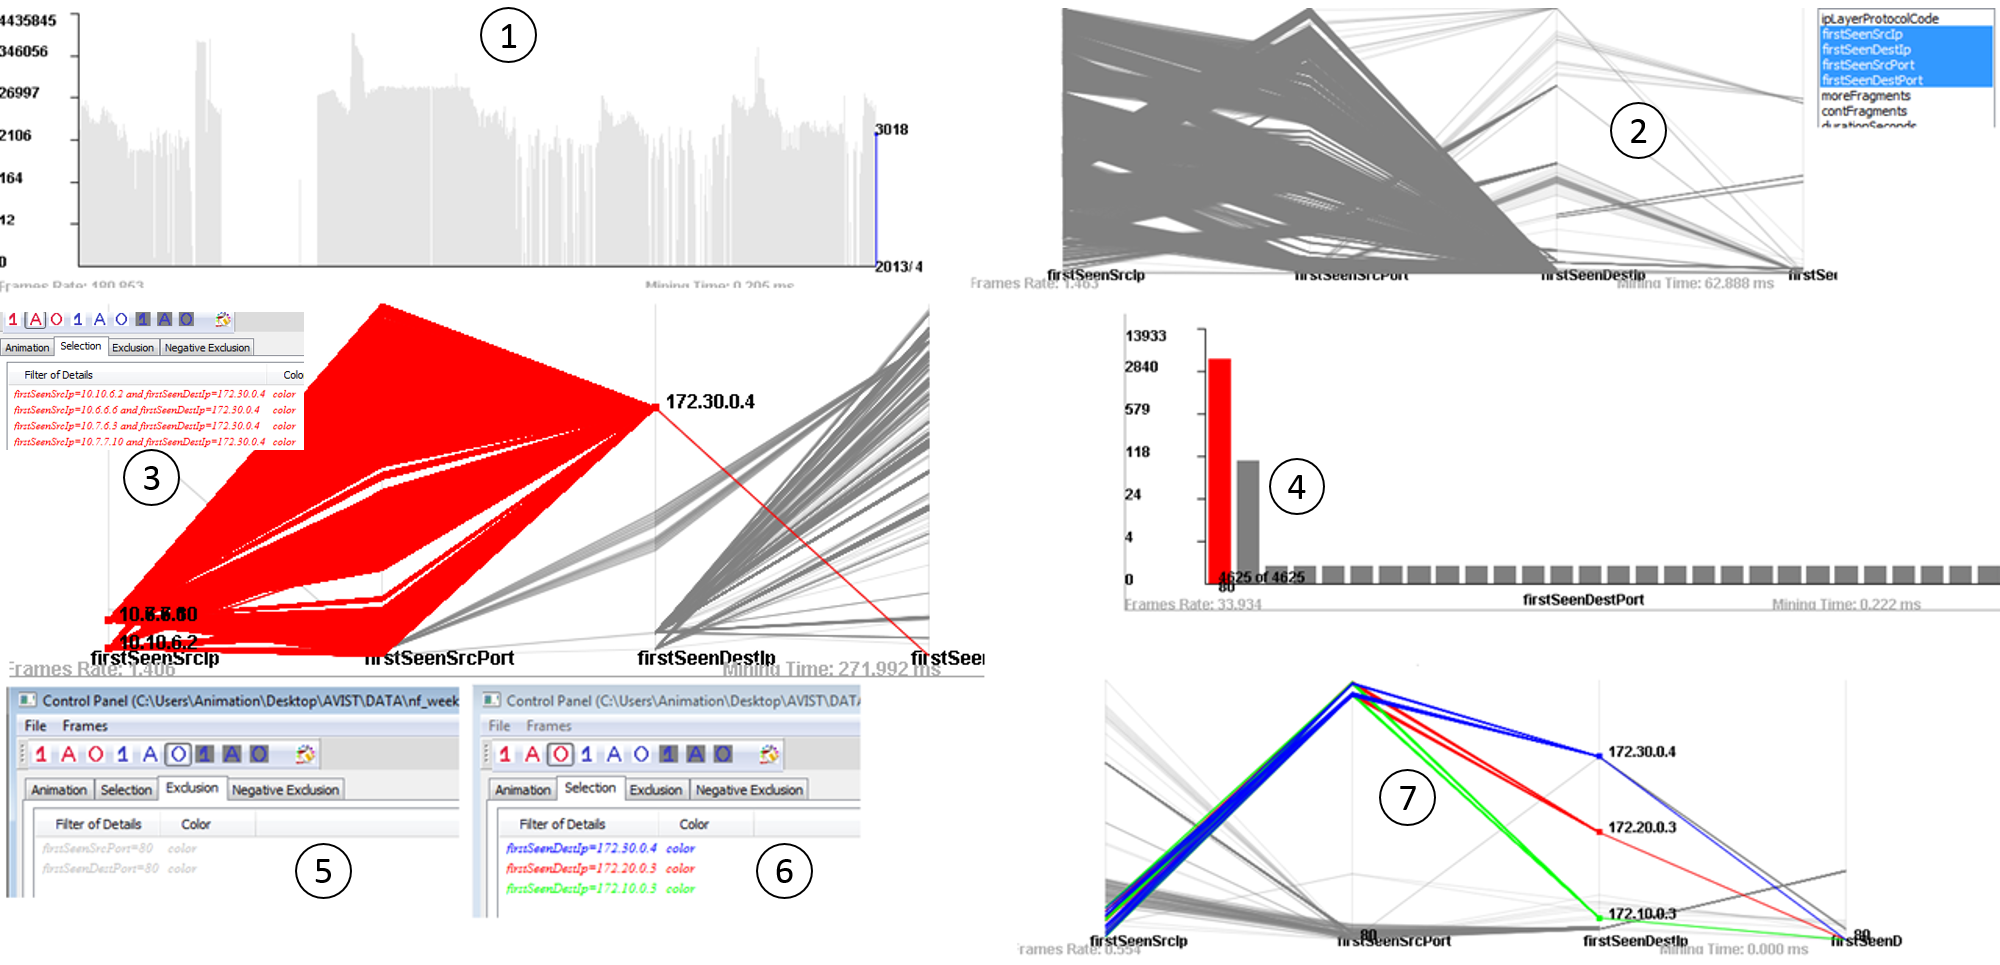
\includegraphics[width=0.9\linewidth]{pic/network2.png}
	\parbox[t]{1.0\columnwidth}{\relax
	}
	%
	\caption{\label{fig:vast}
		This figure shows a usage scenario how AVIST helps analysts for visual exploration of the large network logs. 
		Seven steps are presented in this figure, and Section 6.1 gives more detailed explanations. }
\end{figure*}

\begin{figure*}[htb]
	\centering
	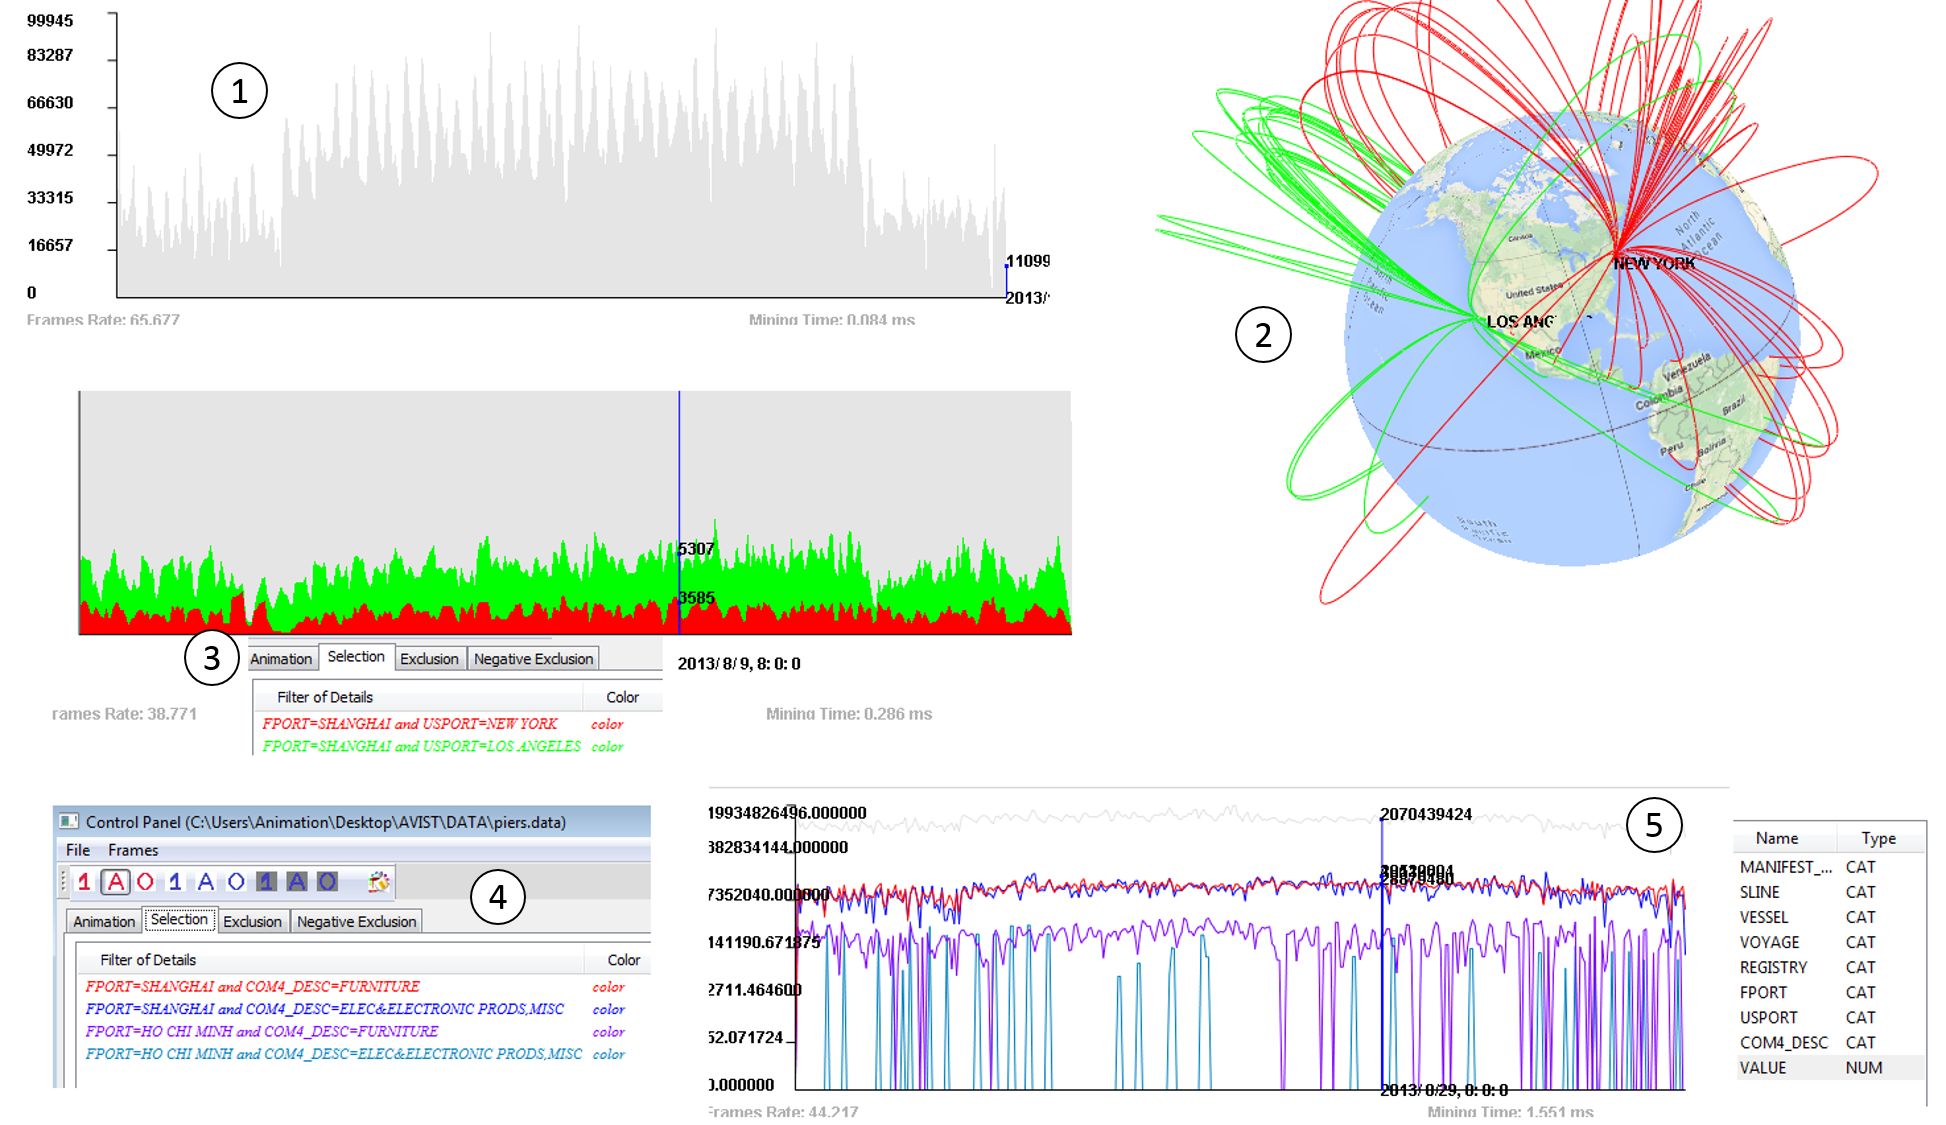
\includegraphics[width=1.0\linewidth]{pic/worldtrade2.png}
	\parbox[t]{1.0\columnwidth}{\relax
	}
	%
	\caption{\label{fig:network}
		This figure shows the usage scenario that analysts use AVIST to visual explore big international trade transactions. The detailed discussions are presented in Section 6.2.}
\end{figure*}

Exploratory visual analysis of network logs is critical for detecting potential cyber threats and network intrusions. VAST 2013 Mini Challenge 3, which targets the analysis of Big Marketing company's network, provides big network traffic logs\footnote{http://vacommunity.org/VAST+Challenge+2013}. One of the datasets is about one week network flow, which includes 46,138,310 records and 16 dimensions.%the total data size is 5.4G

Suppose that Alice is an intelligence analyst. She is assigned to identify the network threats for the Big Marketing company. Firstly, she preprocesses this dataset to obtain the binary data and opens AVIST to load it. Figure~\ref{fig:vast} shows key steps of Alice's visual analytical process. 


\textbf{Data exploration from overview to details.} Firstly, Alice specifies the animation speed and time window size (120 seconds in this example) for automatic animation. The overview of network traffic is visualized in time-series view, shown in subgraph 1. Alice identifies an unusual behavior that the network crashed from 4-2-2013 9:40 am to 4-3-2013 3:26 am. She wants to investigate details before the network crash, so she chooses data dimensions in order of \emph{firstSeenSrcIp}, \emph{firstSeenSrcPort}, \emph{firstSeenDestIp} and \emph{firstSeenDestPort} to generate parallel coordinate plots in subgraph 2. Then she plays animation again and discovers that four source IPs 10.10.6.2, 10.6.6.6, 10.7.6.5, 10.7.7.10 scan the destination IP 172.30.0.4 during 4-2-2013 5:20 am in subgraph 3. 

\textbf{Flexible filtering for revealing hidden patterns.}
Subgraph 4 shows the network traffic distribution of \emph{firstSeenDestPort}. Alice realizes that most of the network records are related with port 80, and she hypothesizes  that these are the normal behavior. She removes these data records with port 80 (subgraph 5) to investigate buried patterns. After the filtering interaction, she plays animation and discovers a port scan activity shown in subgraph 7. She captures this behavior by highlight filters as shown in subgraph 6.  

In this example, Alice iteratively plays animations and tries different filters for identifying potential network threads. She can easily constrains the time and data attributes for capturing any subtle and hidden relationships. Compared with imMens, which preaggregates data before visualization, it cannot provide such flexible interactions, such as cross-domain filtering.
  


\subsection{International Trade Analysis}


Making sense of international trade is important for government and policy makers. With the world economic growth, world trade transactions become large and complex. In this case study, we obtain big international trade transactions from PIERS Global Intelligence Solutions\footnote{https://www.piers.com/}, a private company that provides portfolio analysis for U.S. waterborne trade activity in the world. The dataset is about 2013 US waterborne imports with 10,735,092 records and 10 dimensions. Among 10 dimensions, each data records features the US port code and foreign port code, which illustrates the geospatial information of the dataset.

Suppose that Mike is an economic analyst. He wants to gain insights from the international trade activities. So he  preprocesses and explore this dataset based on AVIST. Figure \ref{fig:network} shows the insights of Mike's visual exploration process.

 
\textbf{Overview exploration.} Mike specifies the time window (86400 seconds or one day) before playing animation. The time-series view shows the overview of the world trades in subgraph 1, which reveals that the activities are clearly separated into four quarters. The second and third quarters has more transactions than others.


\textbf{Hypothesis generation and verification.}
Mike hypothesizes that the international trades may have some spatial patterns. International trades prefer neighboring counties. To verify this, Mike highlights two US ports: Los Angeles (LA) and New York (NY), then he plays animations.
Subgraph 2 shows one snapshot of records with this two ports in virtual globe view, which shows that LA has more trades with pacific countries while NY is more related with Western European. Mike tries to narrow down the data items, which focus on the trades from ShangHai (SH) to LA and NY. He plays animation to refresh the time-series view in subgraph 3. He finds that the trades from SH to LA is roughly twice of trades with NY, which supports  his hypothesis. 

\textbf{Making sense of big data. }
The international trades can character each country's economy. Mike generates four filters to compare the economy of China and Vietnam. He chooses ShangHai port and Ho Chi Minh port for representing these two countries. He emphasizes the trades related about furniture and electronics, as shown in subgraph 4. He is more interested in the money value rather than the number of trades records, so he clicks the value in the listbox and plays animations. Subgraph 5 is the time-series view with four highlighted line charts, which shows that two kinds of trades are more balanced in China, while Vietnam more relies on furniture in its exports. 

